\documentclass[tikz, border=2pt]{standalone}
\usepackage{amsmath}

\begin{document}
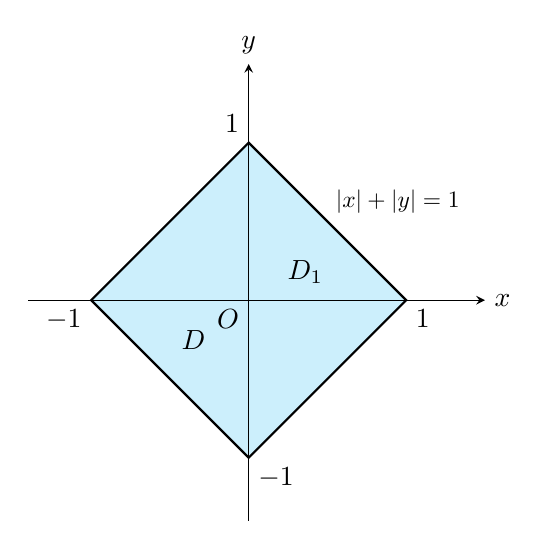
\begin{tikzpicture}[scale=2, >=stealth]
    % D: |x|+|y|<=1
    \fill[cyan!20] (1,0) -- (0,1) -- (-1,0) -- (0,-1) -- cycle;

    \draw[->] (-1.4,0) -- (1.5,0) node[right] {$x$};
    \draw[->] (0,-1.4) -- (0,1.5) node[above] {$y$};

    \draw[thick] (1,0) -- (0,1) -- (-1,0) -- (0,-1) -- cycle;

    \node[below right] at (1,0) {$1$};
    \node[above left] at (0,1) {$1$};
    \node[below left] at (-1,0) {$-1$};
    \node[below right] at (0,-1) {$-1$};
    \node[below left] at (0,0) {$O$};
    \node at (0.36,0.18) {$D_1$};
    \node at (-0.35,-0.25) {$D$};
    \node[above right, scale=0.85] at (0.5,0.5) {$|x|+|y|=1$};
\end{tikzpicture}
\end{document}
